% !TEX root = proposal.tex
\centering
\begin{subfigure}[b]{0.3\textwidth}
  \centering
  \begin{tikzpicture}[->,shorten >=1pt, node distance={15mm}, main/.style = {draw, circle}] 
    \node[main] (3) {$s_3$}; 
    \node[main] (1) [below left of=3] {$s_1$}; 
    \node[main] (2) [below right of=3]{$s_2$}; 

    \path
    (1) edge[bend left=-30] node[above] {\sfrac 1 4} (2)
        edge[bend right=-10] node[below right] {\sfrac 1 2} (3)
        edge[loop left] node[left] {\sfrac 1 4} (1);

    \path
    (2) edge[bend left=40] node[below] {\sfrac 1 4} (1)
        edge[bend left=-10] node[below left] {\sfrac 1 2} (3)
        edge[loop right] node[right] {\sfrac 1 4} (2);

    \path
    (3) edge[bend left=20] node[above right] {\sfrac 1 4} (2)
        edge[bend right=20] node[above left] {\sfrac 1 4} (1)
        edge[loop above,out=80,in=110,looseness=5] node[left=2mm,pos=0.2] {\sfrac 1 2} (3);

  \end{tikzpicture}
  \caption{Markov Process as a graph.}
  \label{fig:mdp_illustration}

\end{subfigure}
\begin{subfigure}[b]{0.69\textwidth}
  \centering
  \begin{align*}
    \pi = \begin{bmatrix}
      \sfrac 1 4 \\
      \sfrac 1 4 \\
      \sfrac 1 2 \\
    \end{bmatrix}, ~
    \Phi & = \begin{bmatrix}
      1 & 0 \\
      0 & -1 \\
      \sfrac{1}{2} (1.05 + \epsilon) & -\sfrac{1}{2} (1.05 + \epsilon)\\
    \end{bmatrix}, ~
    V = \begin{bmatrix}
      1 \\
      1 \\
      1.05 \\
    \end{bmatrix}
  \end{align*}
  \caption{Stationary distribution $\pi$, Value function basis $\Phi$, True state-values $V$}
  \label{fig:mdp_matrix}
\end{subfigure}
